\documentclass{article}
\usepackage[utf8]{inputenc}
\usepackage[super,square]{natbib}
\usepackage{tabularx}
\usepackage{parskip}
\usepackage[margin=1.4in]{geometry}
\usepackage{csquotes}
\usepackage{amsmath}
\usepackage{amsfonts}
\usepackage{amsthm}
\usepackage{amssymb}
\usepackage{hyperref}
\usepackage{graphicx}
\usepackage{float}
\usepackage{textcomp}
\usepackage{multicol}
\usepackage{color,soul}

\usepackage{xcolor}
\usepackage[many]{tcolorbox}
\tcbuselibrary{listings}

\definecolor{light-gray}{gray}{0.95}

% the space reserved between for the ``In'' numbers and the code
\newlength\inwd
\setlength\inwd{1.3cm}


%New colors defined below
\definecolor{codegreen}{rgb}{0,0.6,0}
\definecolor{codegray}{rgb}{0.5,0.5,0.5}
\definecolor{codepurple}{rgb}{0.58,0,0.82}
\definecolor{backcolour}{rgb}{0.95,0.95,0.92}

\definecolor{colab_string}{HTML}{a31515}
\definecolor{colab_kw}{HTML}{a05477}
\definecolor{colab_comment}{HTML}{008000}

%Code listing style named "mystyle"
\lstdefinestyle{mystyle}{
  commentstyle=\color{codegray}, %codegreen},
  keywordstyle=\color{codegreen}, %magenta},
  stringstyle=\color{codepurple}, % codepurple},
  basicstyle=\ttfamily\footnotesize,
  breakatwhitespace=false,         
  breaklines=true,                 
  captionpos=b,                    
  keepspaces=true,                 
  numbers=none,                    
  showspaces=false,                
  showstringspaces=false,
  showtabs=false,                  
  tabsize=2,
}

% \lstset{style=mystyle}

\newcounter{ipythcntr}
\newtcblisting{ipythonnb}[1][\theipythcntr]{
  enlarge left by=\inwd,
  width=\linewidth-\inwd,
  enhanced,
  boxrule=0.4pt,
  colback=light-gray,
  listing only,
  top=0pt,
  bottom=0pt,
  left=4pt,
  listing options={
    style=mystyle,
    basicstyle=\footnotesize\ttfamily,
    language=python,
    escapechar=¢,
    showstringspaces=false,
  },
  overlay={
    \node[
      anchor=north east,
      text width=\inwd,
      font=\footnotesize\ttfamily\color{blue},
      inner ysep=2mm,
      inner xsep=0pt,
      outer sep=0pt
      ] 
      at (frame.north west)
      {\stepcounter{ipythcntr}In [#1]:};
  }
}

% Book headers
\usepackage{fancyhdr}
\pagestyle{fancy}
\fancyhf{}
\fancyhead[L]{\rightmark}
\fancyhead[R]{\thepage}
\renewcommand{\headrulewidth}{0pt}

\title{\vspace{-3cm} \{Artificial, Biological\} Neural Nets }
% \title{\vspace{-3cm} Energy-Based Models and Other Fringe Neural Nets}
\author{}
\date{}

% \comment{
% }

\begin{document}
\maketitle
\vspace{-1.5cm}
\tableofcontents
\newpage

\section{Energy-Based Models}
In an energy-based model (EBM), we make a trade-off for the numerical precision of probabilistic likelihood that comes from normalizing a variable over a density and instead are concerned with finding the dependence between two variables: our input $x$ and compatible $y$ values. In a sense, self-supervised learning (SSL) can simply be understood as learning dependencies. This is in contrast to directly finding or estimating the posterior of a data distribution from large set of samples. EBMs are particularly appealing when making predictions in the presence of uncertainty in high dimensional spaces. They also provide a useful and unifying framework to analyze neural architectures that differ in their use and interpretation of cost function minimization. 

\subsection{Inference on Energy Functions}
We define an energy function as $F: \mathcal X \times \mathcal Y \mapsto \mathcal R$ where $F(x,y)$ describes the level of dependency between $(x, y)$ pairs. Note that the energy is used in inference, not in learning. The inference function is given by the following equation:
\[
\check y = \text{argmin}_y\{ F(x,y)\}
\]

To perform inference, we search this function using gradient descent (or an alternative optimization method) to find compatible $y$’s that minimize the energy function $F$. This is in contrast to the standard approach of performing gradient descent in training.

% \subsection{Latent Variable Energy-Based Models}
In a \textbf{latent variable energy-based model}, the output $y$ depends on $x$ as well as a latent variable $z$ which we do not know the value of. These latent variables can provide auxiliary information and can be thought of as a piece of important information about the output $y$ that is not present in the input $x$. By varying the latent variables over a set, we can let our predicted $y$ vary over the \textit{manifold} of possible predictions. To do inference with latent variables in an EBM, we want to simultaneously minimize the energy function with respect to $y$ and $z$.
\[
\check y, \check z = \text{argmin}_{y,z} E(x,y,z)
\]

\subsection{Normalization of Energy Functions}
EBMs provide an alternative to probability density estimation by learning a manifold to compute the dependency of variables. In doing so, they provide a method to describe probabilistic and non-probabilistic approaches to learning without needing to estimate the normalization constant in probabilistic models, increasing flexibility of the model.

The \textbf{Gibbs-Boltzmann distribution} was originally used in thermodynamics to find the probability that a system will be in a certain state $i$ as a function of that state's energy $\epsilon_i$ and the temperature $T$ of the system. Here $\propto$ indicates proportionality under a constant and $k$ is known as Boltzmann's constant.  
\begin{align*}
    p_{i} &\propto \exp \bigg ( -{\frac {\varepsilon_{i}}{kT}} \bigg )\\
     &= \exp \bigg( - \frac{E(x, y)}{kT} \bigg )
\end{align*}

Energies can then be thought of as being \textit{unnormalized negative log probabilities}. That is, we may use the Gibbs-Boltzmann distribution to convert an energy function to its equivalent probabilistic representation after normalization, i.e. $P(y \mid x)$. 

The derivation introduces a $\beta$ term which is the inverse of temperature $T$, so as $\beta \rightarrow \infty$ the temperature goes to zero. $\beta$ is a positive constant that needs to be calibrated to fit the model. A larger $\beta$ value produces a more fluctuate model while a smaller $\beta$ gives a smoother model. 
\[
    P(y, z \mid x) = \frac{\exp(-\beta E(x,y,z)) }{ \int_y \int_z \exp(\beta E(x, y, z))} 
\]
Recall, \textit{marginalisation} is a method that sums over the possible values of one variable to determine the marginal contribution of another. $P(y \mid x)$ is just an application of the Gibbs-Boltzmann formula with latent variables $z$ being marginalized implicitly through integration, i.e. $P(y \mid x) = \int_z P(y,z | x)$. Then,
\begin{align*}
    P(y \mid x) &= \frac{ \int_z \exp(-\beta E(x,y,z)) }{ \int_y \int_z \exp(-\beta E(x, y, z))} \\
    &= \frac{
        \exp \bigg [  -\beta (-\frac{1}{\beta} \log  \int_z \exp(-\beta E(x,y,z)) ) \bigg ]
    }{
        \int_y \exp \bigg [  -\beta (-\frac{1}{\beta} \log  \int_z \exp(-\beta E(x,y,z)) ) \bigg ]
    }
\end{align*}

\subsection{Free Energy}

When $\beta \rightarrow \infty$, we see that $\check{y} = \text{argmin}_{y} E(x,y)$. So we can redefine our energy function as an equivalent function using $F_\beta$,
\begin{align*}
    F_{\infty} (x,y) &= \text{argmin}_z E(x,y,z)\\
    F_{\beta} (x,y) &= -\frac{1}{\beta} \log \int_z \exp(-\beta E(x,y,z)).
\end{align*}

In physics, $F_\beta$ is known as the \textbf{free energy} -- so $E$ is the energy, and $F$ is free energy. If we have a latent variable model and want to eliminate the latent variable $z$ in a probabilistically correct way, we just need to redefine the energy function in terms of $F_\beta$,

\[
    P(y \mid x) = \frac{ \exp(-\beta F_\beta(x,y,z)) }{ \int_y \exp(-\beta F_\beta(x, y, z))}. \\
\]

\subsection{Training Energy Functions}

There are two classes of learning models to train an EBMs in order to parameterize $F(x, y)$:

\begin{enumerate}
    \item \textbf{Contrastive methods} push down the energy of training data points, $F(x_i, y_i)$, while pushing up energy everywhere else, $F(x_i, y')$. Types of contrastive methods differ in the way they pick the points to push up.
    
    For an example of this method, see the section on Generative Adversarial Networks.
    
    \item \textbf{Regularized latent variable methods} build energy function $F(x, y)$ so that the volume of low energy regions is limited or minimized by applying regularization. Types of architectural methods differ in the way they limit the information capacity of the code.
    
    For an example of this method, see the section on Variational Autoencoders.
\end{enumerate}

Examples of constrastive learning methods include Contrastive Divergence, Ratio Matching, Noise Contrastive Estimation, and Minimum Probability Flow. The term \textit{contrastive sample} is often used to refer to a data point causing an energy pull-up, such as the incorrect $y$'s in supervised learning and points from low data density regions in unsupervised learning.

TODO: add sections on Contrastive embedding, Sparse Coding, Contrastive Divergence.

\subsection{Combining Densities}
There are three ways to combine probability density models:
\begin{enumerate}
    \item \textbf{Mixture} -- Take a weighted average of the distributions. The mixture can never be sharper than the individual distributions, making this is a very weak way to combine models. 
    \item \textbf{Product} -- Multiply the distributions at each point and then renormalize. This is exponentially more powerful than a mixture. The normalization makes maximum likelihood learning difficult, but approximations allow us to learn anyway. 
    
    \item \textbf{Composition} -- Use the values of the latent variables of one model as the data for the next model. This works well for learning multiple layers of representation, but only if the individual models are undirected.
\end{enumerate}

It is possible to combine multiple latent-variable models of the same data by multiplying their probability distributions together and then renormalizing. This way of combining individual ``expert” models makes it hard to generate samples from the combined model but easy to infer the values of the latent variables of each expert, because the combination rule
ensures that the latent variables of different experts are conditionally independent when given the data. This technique is known as the \textbf{product of experts} (PoE).

As we've seen, energy-based models represent probability distributions over data by assigning an unnormalized probability scalar, i.e. an energy, to each input data point. This provides useful modeling flexibility since any arbitrary model that outputs a real number given an input can be used as an energy model. Since each model represents an unnormalized probability distribution, models can be naturally combined through product of experts or other hierarchical models.

\subsection{Directed Models vs. Energy-Based Models}
\begin{figure}[H]
    \centering
    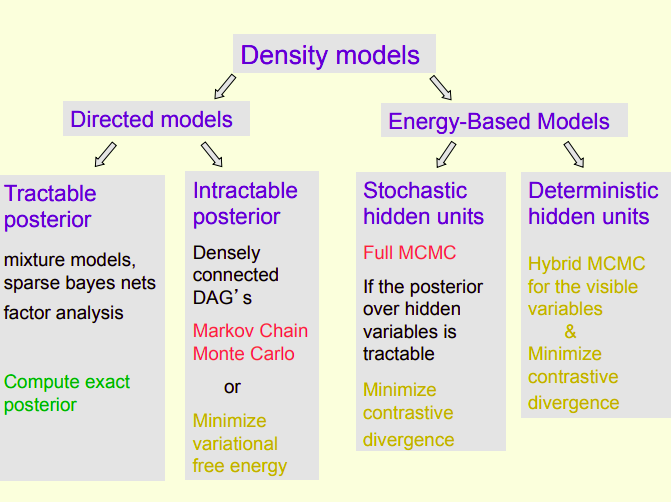
\includegraphics[width=12cm]{dag-ebm.png}
\end{figure}

There are two categories of density models:
\begin{enumerate}
    \item Stochastic generative models using directed acyclic graphs (see section on Bayes Networks). Generation from this type of model is easy, inference can be hard, and learning is easy after inference. 
    \[
        P(v) = \sum_h P(h)P(v | h)
    \]
    where $v$ are the visible units and $h$ are the hidden units.
    
    \item Energy-based models that associate an energy with each data vector. Generation this type of model is hard, inference can be easy, and learning is typically hard but varies.
    \[
        P(v, h) = \frac{\exp(-E(v, h))}{\sum_{u, g} \exp(-E(u, g))}
    \]
    The probability of a joint configuration over both visible and hidden units depends on the energy of that joint configuration compared with the energy of all other joint configurations.
    \[
         P(v) = \frac{\sum_{h} \exp(-E(v, h))}{\sum_{u, g} \exp(-E(u, g))}
    \]
    The probability of a configuration of the visible units is the sum of the probabilities of all the joint configurations that contain it. 
\end{enumerate}


Probabilities can be understood as integrating over a density. In Bayesian analysis, many of the densities are not analytically tractable or have a posterior that is expensive to compute. When it is intractable, we can try to programmatically simulate a random variable with the given density. 

\textbf{Markov chain Monte Carlo (MCMC)} are algorithmic methods for sampling from a probability distribution that is represented as graphical model, i.e. a Markov chain. Under certain conditions, we can generate a memoryless (Markovian) process in the form of an ensemble of Markov Chains that has the same limiting distribution as the random variable that we're trying to simulate. Because of the memoryless property, a large number of random walks through the chains using simulations of the random variable will represent correlated independent samples. Eventually this process will converge to an equilibrium distribution and produce an estimate of an otherwise intractable posterior.

Surprisingly, it is unnecessary to allow the simulated physical process to reach the equilibrium distribution. If we start the process at an observed data vector and run it for a few steps, we can generate a ``confabulation” that works well for adjusting the weights. If the Markov chain starts to diverge from the data in a systematic way, we already have evidence that the model is imperfect and that it can be improved (in this local region of the data space) by reducing the energy of the initial data vector and raising the energy of the confabulation. 

The \textbf{contrastive backpropagation} learning procedure cycles through the observed data vectors adjusting each weight by:
\[
    \triangledown w_{ij} = a \bigg (  - \frac{\partial E(x)}{\partial w_{ij}} +  \frac{E(\hat x)}{\partial w_{ij}} \bigg)
\]
where $a$ is a learning rate and $\hat x$ is the confabulation produced by starting at $x$ and noisily following the gradient of the energy surface for a few steps.


\section{Early Models of the Mind}

\subsection{Bayesian Networks}

The basis of all Bayesian statistics can be interpreted through \textbf{Bayes' Theorem}, simply stated as $\text{posterior}\propto \text{prior} \times \text{likelihood}$, where $\propto$ indications proportionality. Equivalently, this can be expressed with conditional probabilities as,
\[
P(A\mid B)={\frac {P(B\mid A)P(A)}{P(B)}}.
\]

A \textbf{Bayesian Network} is a directed acyclic graph that represents a factorization of the joint probability of all random variables.  If the random variables are $X_{1},\ldots ,X_{n}$ then the joint distribution factors into a product of conditional distributions, 
\[
    P(X_{1},\ldots ,X_{n}) = \prod_{i=1}^{n}P(X_{i} | {\text{ pa}}(X_{i}))
\]
where ${\text{pa}}(X_{i})$ is the set of parents of node $X_{i}$. Classical neural networks and hidden Markov Models are a form of Bayesian belief networks. A typical analysis under the Bayesian model is outlined below:


\begin{enumerate}
    \item Define the prior distribution that incorporates subjective beliefs about a parameter. If the prior is uninformative, the posterior is data-driven. If the prior is informative, the posterior is a mixture of the prior and the data.
    
    \item Collect data. The more informative the prior, the more data you need to ``change" your beliefs. With a lot of data, the data will dominate the posterior distribution.
    
    \item Update the prior distribution with the collected data using Bayes' theorem to obtain a posterior distribution. The posterior distribution represents the updated beliefs about the parameter after having seen the data. In most cases, the posterior distribution has to be found via MCMC simulations.
    
    \item Analyze the posterior distribution and summarize it (i.e. by describing its mean, median, standard deviation, quantiles, etc.)
\end{enumerate}

\subsection{Binary Hopfield Networks and Hebbian Theory}

The \textbf{Hopfield network} is a complete undirected graph made of binary threshold neurons, usually having values of either 1 or -1, with all pairs of units connected by symmetric weighted edges. Hopfield networks serve as content-addressable memory and provide a model for understanding \textbf{associative memory} in humans.

The constraint that weights are symmetric guarantees that the energy function decreases monotonically, guaranteeing that descending its manifold will converge to a local minimum. The energy, $E$, can be described in terms of scalar values associated to each of the states of the network,
\[
    E = -\frac{1}{2} \sum_{i,j} w_{ij} s_i s_j + \sum_i \theta_i s_i.
\]
where $w_{ij}$ is the weight of the connection from unit $i$ to unit $j$, $s_{i}$ is the state of the unit $i$, and $\theta_{i}$ is the threshold. Unlike in perceptron training, the thresholds of the neurons are never updated.

Training a Hopfield network involves lowering the energy of states that we want the network to remember. The network will converge to a remembered state if it is given only part of the queried state, i.e. given a distorted pattern it can recover a memorized one that is most similar. Much like our own memory, the network may retrieve the wrong pattern, known as a spurious pattern, from the wrong local minimum instead of the intended pattern, known as retrieval states, at the expected local minimum. For each stored pattern $x$, the negation $-x$, known as a spurious pattern, is also stored. For a network with $n$ neurons, the storage capacity is given as, 
\[
    C\cong {\frac {n}{2\log _{2}n}} \approxeq 0.15n. 
\]

Hopfield networks called \textbf{dense associative memory} (DAM) models use an energy function that can be expressed as the sum of interaction functions $F$ of the form $F(x) = x^n$ and, thereby, achieve a storage capacity proportional to $d^{n-1}$ in a d-dimensional space.

Updating units in the Hopfield network can be done one at a time, in a biologically plausible and asynchronous way, or they can be updated synchronously, all at the same time. Updating is performed using the following rule:
\[
s_{i} \leftarrow \left\{
    {
    \begin{array}{ll}+1&{\mbox{if }} \displaystyle \sum _{{j}}{w_{{ij}}s_{j}}\geq \theta _{i},\\-1&{\mbox{otherwise.}}\end{array}
    }\right.
\]
The updating rule implies that neurons attract or repel each other in state space, i.e. the values of neurons will converge if the weight between them is positive or they will diverge if the weight is negative. Under repeated updates, the network will eventually converge to a stable state which is a local minimum or basin of attraction in the energy function. 

A learning rule is used to store information in the memory. It must follow the constraints of only being local to a neuron and its adjacent neurons and must be incremental, meaning that updating weights to store a new pattern must be dependent on values of the previously stored information. These rules enforce a sort of biologically plausibility on the network but have been altered to improve functionality (see section on continuous Hopfield networks).

The \textbf{Hebbian theory} of synaptic plasticity is closely related to the constraints of this model. The Hebbian rule is often summarized as ``Neurons that fire together, wire together", and is both local and incremental like the standard Hopfield network. When learning $n$ binary patterns where $\epsilon_{i}^{\mu }$ represents bit $i$ from pattern $\mu$, the Hebbian learning rule is expressed as,
\[
 w_{{ij}}={\frac  {1}{n}}\sum _{{\mu =1}}^{{n}}\epsilon _{{i}}^{\mu }\epsilon _{{j}}^{\mu }
\]

\textbf{Spike-timing-dependent plasticity} (STDP) is a biological process that adjusts the strength of connections between neurons in the brain. The process adjusts the connection strengths based on the relative timing of a particular neuron's output and input action potentials (or spikes). 

Experiments that stimulated two connected neurons with varying interstimulus asynchrony confirmed the importance of temporal precedence implicit in Hebb's principle: the presynaptic neuron has to fire just before the postsynaptic neuron for the synapse to be potentiated. In addition, it has become evident that the presynaptic neural firing needs to consistently predict the postsynaptic firing for \textbf{synaptic plasticity} to occur robustly.


\subsection{Free Energy Principle and Predictive Coding}
The \textbf{free energy principle}, introduced by neuroscientest Karl Friston, generalizes a formal description of how systems minimize a free energy function of their internal states in an attempt to generate beliefs about hidden states in their environment.

In terms of the brain, we are given sensory information in current and past inputs while neurons are continuously performing inference by updating into configurations that better explain the observed sensory data. This theory of brain function, in which the brain is constantly generating and updating a mental model of the world, is known as \textbf{predictive coding}.

We can represent these configuration of internal neurons as continuous valued latent variables that correspond to averaged voltage potential across time, spikes, and possibly neurons in the same cortical minicolumn. Thus, neural computation corresponds to approximate inference and error back-propagation at the same time. It has been shown that the predictive coding model is able to approximate backpropagation along arbitrary computation graphs, making it biologically plausible but is still computationally infeasible with our current hardware. An alternative \textbf{neuromorphic} hardware or wetware architecture might someday be able to run massively parallelized computations only using local rules that may outperform backpropagation through time methods.

When reformulated using a generalized notation, active inference in the brain can be formally described on the tuple $(\Omega ,\Psi ,S,A,R,q,p)$. 
\begin{itemize}
    \item \textbf{A sample space $\Omega$  –} from which random perturbations $\omega \in \Omega$  are drawn
    \item \textbf{Hidden or external states $\Psi:\Psi\times A \times \Omega \to \mathbb{R}$} – that cause sensory states and depend on action
    \item \textbf{Sensory states $S:\Psi \times A \times \Omega \to \mathbb{R}$} – a probabilistic mapping from action and hidden states
    \item \textbf{Action $A:S\times R \to \mathbb{R}$} – that depends on sensory and internal states
    \item \textbf{Internal states $R:R\times S \to \mathbb{R}$} – that cause action and depend on sensory states
    \item \textbf{Generative density $p(s,\psi \mid m)$} – over sensory and hidden states under a generative model $m$
    \item \textbf{Variational density $q(\psi \mid \mu )$} – over hidden states $\psi \in \Psi$ that is parameterised by internal states $\mu \in R$
\end{itemize}

This closely resembles energy-based learning models, where predicted outputs $y$ would would be equivalent to sensory events $s$, latent variables $z$ would be equivlent to hidden states $\psi$ and the known input $x$ would be the generative model $m$. The objective is to maximise model evidence $P(s\mid m)$ or minimize \textit{surprise}, $-\log P(s\mid m)$.
\begin{align*}
    \underset {\mathrm {free-energy} }{\underbrace {F(s,\mu )}} 
    &={\underset {\mathrm {energy} }{\underbrace {E_{q}[-\log p(s,\psi \mid m)]} }}-{\underset {\mathrm {entropy} }{\underbrace {H[q(\psi \mid \mu )]} }}\\
    &={\underset {\mathrm {surprise} }{\underbrace {-\log p(s\mid m)} }}+{\underset {\mathrm {divergence} }{\underbrace {D_{\mathrm {KL} }[q(\psi \mid \mu )\parallel p(\psi \mid s,m)]} }}\\
    &\geq {\underset {\mathrm {surprise} }{\underbrace {-\log p(s\mid m)} }}
\end{align*}


\subsection{Helmholtz Machines and the Wake--Sleep Algorithm}
The notion that self-organising biological systems are continuously updating themself in order to minimize variational free energy was derived from the work of the German physicist Helmholtz. In particular, acknowledgments are made to Helmholtz's conception of \textit{unconscious inference}, which encapsulates the view of the human perceptual system as a statistical inference engine whose core function is to infer the probable causes of sensory input.

\textbf{Helmholtz machines} are artificial neural networks that, through many cycles of sensing and generative dreaming, gradually learn to how to converge their dreams into reality. In this process they create a succinct internal model of a fluctuating world, making them highly suitable for unsupervised learning tasks. The Helmholtz machine contains two networks, a bottom-up \textit{recognition} network that takes an external observation as input and produces a distribution over hidden variables, and a top-down \textit{generative} network that generates values of the hidden variables and the data itself. 

The \textbf{Wake-Sleep algorithm}, used for training, consists of two phases:
\begin{enumerate}
    \item In the wake phase, neurons are driven by recognition connections, and generative connections are adapted to increase the probability that they would reconstruct the correct activity vector in the layer below.
    
    \item In the sleep phase, neurons are driven by generative connections, and recognition connections are adapted to increase the probability that they would produce the correct activity vector in the layer above.
\end{enumerate}

\subsection{Autoencoders}
The Helmholtz Machine served as an important precursor for \textbf{autoencoder networks (AE)} which are also a discriminative model used for making predictions and are similarly composed of a sequence of two networks: one for encoding inputs (analogous to the recognition network) and another for decoding outputs (analogous to the generative network). The encoder network learns a representation of the data by mapping data to a compressed or latent space and then training the decoder to generate an output that minimizes the reconstruction loss. 

On its own, this model would be prone to copying all the input features into the hidden layer and passing it directly as the output, essentially behaving like an identity function and not learning anything. This is avoided by applying an \textit{information bottleneck} by feeding the coded input into hidden layers of lower dimension known as \textit{under-complete layers}. An under-complete layer cannot behave as an identity function simply because the hidden layer doesn't have enough dimensions to copy the original input. 

An \textit{affine} transformation preserves lines and parallelism, i.e. it's a linear function with a translation constant. A very simple form of an AE does the following:

\begin{enumerate}
    \item In the encoder stage, the autoencoder takes in an input $x \in \mathbb R^n$ and applies an affine transformation, $W_h \in \mathbb R^{d\times n}$, resulting in an intermediate hidden layer $h \in \mathbb R^d$:
    
    $h = f(W_h x + b_h)$, where $f$ is an element-wise activation function and $h$ is called the code.
    
    \item In the decoder stage another affine transformation, defined by $W_x  \in \mathbb R^{n\times d}$, produces the output $\hat{x} \in \mathbb R^n$, which is the model's prediction/reconstruction of the input:
    
    $\hat{x} = g(W_x h + b_x)$, where $g$ is an activation function.
\end{enumerate}

Instead of using the wake-sleep algorithm as was done in Helmholtz machines, autoencoders are trained using backpropagation. \textit{Cross-Entropy} can be used as a loss function $\ell$ when the input is categorical and the \textit{Mean Squared Error Loss} can be used when the input is real-valued. The overall loss for the dataset is given as the average per sample loss,
\[
    L = \frac{1}{m}\sum_{j=1}^m \ell (x^{(j)}, \hat x^{(j)}).
\]


Interpreted as an energy-based model, we train the system to produce an energy function that grows quadratically as the corrupted data moves away from the data manifold. For a \textit{denoising autoencoder}, training can be done using \textbf{contrastive divergence (CD)} to handle the uncountable ways to corrupt a piece of data in high-dimensional space. 

In a continuous space, CD first picks a training sample $y$ and lowers its energy. For that sample, it uses a gradient-based process to move downward on the energy surface with noise. If the input space is discrete, it can instead perturb the training sample randomly to modify the energy. If the energy becomes lower, the perturbed sample is kept, otherwise, it's discarded with some probability. Continuing this process will eventually lower the energy of $y$. We can then update the parameter of our energy function by comparing $y$ and the contrasted sample $\bar y$ using a loss function.

\begin{minipage}{\textwidth}
\vspace{8pt}
\emph{Model}
\vspace{8pt}
\begin{ipythonnb}
class Autoencoder(nn.Module):
    def __init__(self):
        super().__init__()
        self.encoder = nn.Sequential(
            nn.Linear(n, d),
            nn.Tanh(),
        )
        self.decoder = nn.Sequential(
            nn.Linear(d, n),
            nn.Tanh(),
        )

    def forward(self, x):
        x = self.encoder(x)
        x = self.decoder(x)
        return x
\end{ipythonnb}
\end{minipage}

\begin{minipage}{\textwidth}
\vspace{8pt}
\emph{Training}
\vspace{8pt}
\begin{ipythonnb}
model = Autoencoder().to(device)
criterion = nn.MSELoss()
learning_rate = 1e-3
optimizer = torch.optim.Adam(
    model.parameters(),
    lr=learning_rate,
)
num_epochs = 20
for epoch in range(num_epochs):
    for data in dataloader:
        img, _ = data
        img = img.to(device)
        img = img.view(img.size(0), -1)
        # ===================forward=====================
        output = model(img)  
        loss = criterion(output, img.data)
        # ===================backward====================
        optimizer.zero_grad()
        loss.backward()
        optimizer.step()
    # ===================log========================
    print(f'epoch [{epoch + 1}/{num_epochs}], loss:{loss.item():.4f}')
\end{ipythonnb}
\end{minipage}

\section{Modern Generative Models}

The development of sophisticated learning procedures have been built on a few key assumptions of early models of the brain and have turned out to be highly effective. The assumptions are as follows:
\begin{enumerate}
    \item The brain is a hierarchical or sequential composition of layered networks that specialize in certain functionality but are closely integrated with one another.
    \item There likely exists a network that processes complex sensory or semi-structured input into encoded or latent data before communicating it to layers above it, i.e. in a bottom-up manner. This latent representation of observations of reality can be thought of as a symbolic and denoised representation of the world.
    \item There exists a network that learns from latent representations and attempts to generate useful predictions of the world in a top-down down manner. This can be hypothesized as being closely related to processes that occur in our mind during imagination and when dreaming.
    \item  Although incomprehensible to us, structured data and knowledge appears to exist on a manifold in high-dimensional space. Supervised-learning is a form of probing and exploring this hidden structure.
\end{enumerate}

\subsection{Variational Autoencoders}
Variational Autoencoders (VAE) are a type of generative models that aim to simulate the data generative process. VAEs have conceptual similarities to autoencoders, but have very different formulations. The main difference between VAEs and AEs is that VAEs are designed to create a better latent space for capturing underlying causal relations that in turn enables them to perform better in the generative process.

\begin{enumerate}
    \item In the encoder stage, the input $x$ is passed to the encoder. Instead of generating a hidden representation of the the code $h$, as was done in an AE, the code in a VAE is comprised of two things: the mean, $\mathbb{E}(z)$, and the variance, $\mathbb{V}(z)$, where $z$ is the latent random variable following a \textit{Gaussian distribution}. (Other distributions can be used, but a Gaussian is most common in practice. A reparameterization trick is used when sampling $z$, this is outlined in more detail below.)
    
    The encoder will be a function from $\mathcal{X}$ to $\mathbb{R}^{2d} : x \mapsto {h}$, where $h$ represents the concatenation of $\mathbb{E}({z})$ and $\mathbb{V}({z})$.
    
    \item In the sampler stage, $z$ is sampled from the above distribution parametrized by the encoder. Specifically, $\mathbb{E}({z})$ and $\mathbb{V}({z})$ are passed into a sampler to generate the latent variable $z$.
    
    \item In the decoder stage, $z$ is passed into the decoder to generate $\hat{x}$.
    
    The decoder will be a function from $\mathcal{Z}$ to $\mathbb{R}^{n}: z \mapsto \hat{x}$.
\end{enumerate}

To obtain $z$, we can't simply sample from the Gaussian distribution because when we do gradient descent to train the VAE model, we won’t know how to do backpropagation through the sampling module. Instead, we use the \textbf{reparameterization trick}: $z = \mathbb E (z) + \epsilon \odot \mathbb V(z)$ where $\epsilon\sim \mathcal{N}(0, {I}_d)$. Now backpropagation in training is possible, the gradients will go through the element-wise multiplication and addition in the above equation.

To train the VAE, we want to minimize a loss function which will be composed of a reconstruction term as well as a regularization term. Regularization is done by using a penalty term $\ell_{KL}(z, \mathcal N(0, I_d))$. Without this term, the VAE will act like a standard autoencoder which may lead to overfitting and we won’t have the generative properties we desire.

We can write the loss as $\ell(x, \hat x) = \ell_{reconstruction} + \ell_{KL}(z, \mathcal N(0, I_d))$ where,
\[
    \ell_{reconstruction}= 
    \begin{cases}
        -\displaystyle \sum_{i=1}^{n}[x_i \log(x_i) + (1-x_i)\log(1-\hat x_i)] , & \text{for binary inputs}\\ \\ 
        \ \ \ \displaystyle \frac{1}{2}||x -\hat x||, & \text{for real-valued inputs}
    \end{cases}
\]

In general, to go from the latent space to input space during the generative process, we will need to either learn the underlying distribution of the latent code or enforce some structure on the space. In a VAE the regularization term is used to enforce a specific Gaussian structure on the latent space. The penalty term is the \textit{relative entropy} which is a measure of the distance between two distributions: the latent variables sampled from the Gaussian distribution and the standard normal distribution.
\[
    \ell_{KL}(z, \mathcal N(0, I_d)) = 
    \frac{\beta}{2}\sum_{i=1}^{d}(\mathbb{V}(z_i) - \log[\mathbb{V}(z_i)] - 1 + \mathbb{E}(z_i)^2 )
\]

Interpreted as an energy-based model, Variational Autoencoders have an architecture similar to \textit{Regularized Latent Variable EBM} where the flexibility of the latent variable is constrained in order to prevent an energy function from being 0 everywhere. This happens because every true output $y$ can be perfectly reconstructed from input $x$ with an appropriately chosen $z$. To solve this, we may limit the information capacity of the latent variable $z$ through regularization,
\[
    E(x,y,z) = C(y, \text{Dec}(\text{Pred}(x), z)) + \lambda R(z),
\]
where Dec is the decoder, Pred is the predictor, and $R$ is the regularization function. The value of $\lambda$ controls how much we limit the volume of space of $z$ which will, in turn, control the space of $y$ that has low energy. In a VAE, $R$ adds noise to $z$ while limiting its \textit{$L_2$ norm} which will limit its information content. Recall, The $L_2$ norm calculates the euclidean distance of a vector coordinate from the origin of the vector space.

The latent variable $z$ is not computed by minimizing the energy function with respect to $z$. Instead, the energy function is viewed as sampling $z$ randomly according to a distribution whose logarithm is the cost that links it to $\overline z$. The distribution is a Gaussian with mean $\overline z$ and this results in Gaussian noise being added to $\overline z$.

The effects of regularization with Gaussian noise can be visualized as connecting the code vectors spheres $\overline z$ with a spring. The unregularized vectors have a tendency to grow as large as possible in an attempt to disperse the noise on $z$ and to prevent overlapping spheres that would cause reconstruction loss. Connecting them with a loose spring encourages the spheres to cluster around the data manifold without pushing them to converge at the origin.

\begin{minipage}{\textwidth}
\vspace{8pt}
\emph{Model}
\vspace{8pt}
\begin{ipythonnb}
d = 20
class VAE(nn.Module):
    def __init__(self):
        super().__init__()
        self.encoder = nn.Sequential(
            nn.Linear(784, d ** 2),
            nn.ReLU(),
            nn.Linear(d ** 2, d * 2)
        )
        self.decoder = nn.Sequential(
            nn.Linear(d, d ** 2),
            nn.ReLU(),
            nn.Linear(d ** 2, 784),
            nn.Sigmoid(),
        )

    def reparameterise(self, mu, logvar):
        if self.training:
            std = logvar.mul(0.5).exp_()
            eps = std.data.new(std.size()).normal_()
            return eps.mul(std).add_(mu)
        else:
            return mu

    def forward(self, x):
        mu_logvar = self.encoder(x.view(-1, 784)).view(-1, 2, d)
        mu = mu_logvar[:, 0, :]
        logvar = mu_logvar[:, 1, :]
        z = self.reparameterise(mu, logvar)
        return self.decoder(z), mu, logvar
\end{ipythonnb}
\end{minipage}

\begin{minipage}{\textwidth}
\vspace{8pt}
\emph{Loss Function}
\vspace{8pt}
\begin{ipythonnb}
def loss_function(x_hat, x, mu, logvar):
    BCE = nn.functional.binary_cross_entropy(
        x_hat, x.view(-1, 784), reduction='sum'
    )
    KLD = 0.5 * torch.sum(logvar.exp() - logvar - 1 + mu.pow(2))

    return BCE + KLD
\end{ipythonnb}
\end{minipage}

\begin{minipage}{\textwidth}
\vspace{8pt}
\emph{Training and Testing}
\vspace{8pt}
\begin{ipythonnb}
model = VAE().to(device)
epochs = 10
codes = dict('mu'=list(), 'logvar'=list(), 'y'=list())
for epoch in range(0, epochs + 1):
    # Training
    if epoch > 0:  # test untrained net first
        model.train()
        train_loss = 0
        for x, _ in train_loader:
            x = x.to(device)
            # ===================forward=====================
            x_hat, mu, logvar = model(x)
            loss = loss_function(x_hat, x, mu, logvar)
            train_loss += loss.item()
            # ===================backward====================
            optimizer.zero_grad()
            loss.backward()
            optimizer.step()
        # ===================log========================
        print(f'Epoch: {epoch} Average loss: {train_loss / len(train_loader.dataset):.4f}')
    
    # Testing
    means, logvars, labels = list(), list(), list()
    with torch.no_grad():
        model.eval()
        test_loss = 0
        for x, y in test_loader:
            x = x.to(device)
            # ===================forward=====================
            x_hat, mu, logvar = model(x)
            test_loss += loss_function(x_hat, x, mu, logvar).item()
            # =====================log=======================
            means.append(mu.detach())
            logvars.append(logvar.detach())
            labels.append(y.detach())
    # ===================log========================
    codes['mu'].append(torch.cat(means))
    codes['logvar'].append(torch.cat(logvars))
    codes['y'].append(torch.cat(labels))
    test_loss /= len(test_loader.dataset)
    print(f'Test set loss: {test_loss:.4f}')
\end{ipythonnb}
\end{minipage}


\subsection{Deep Boltzman Machines}
TODO

% If we connect binary stochastic neurons in a directed acyclic graph we get a Sigmoid Belief
% Net (Radford Neal 1992).

% If we connect binary stochastic neurons using symmetric connections we get a Boltzmann
% Machine (Hinton \& Sejnowski, 1983).  If we restrict the connectivity in a special way, it is easy to learn a Boltzmann machine. 

% Boltzmann distribution
% https://arxiv.org/pdf/1606.01651.pdf

% Contrastive divergence

% Deep Belief Network

\subsection{Generative Adversarial Networks}

% GANs can be interpreted in two complementary ways. In the first interpretation, the key component
% is the generator, and the discriminator plays the role of a trainable objective function. Let us imagine
% that the data lies on a manifold. Until the generator produces samples that are recognized as being on
% the manifold, it gets a gradient indicating how to modify its output so it could approach the manifold.
% In such scenario, the discriminator acts to punish the generator when it produces samples that are
% outside the manifold. This can be understood as a way to train the generator with a set of possible
% desired outputs (e.g. the manifold) instead of a single desired output as in traditional supervised
% learning.
% For the second interpretation, the key component is the discriminator, and the generator is merely
% trained to produce contrastive samples. We show that by iteratively and interactively feeding contrastive samples, the generator enhances the semi-supervised learning performance of the discriminator (e.g. Ladder Network),

The basic idea of \textbf{generative adversarial network (GAN)} is to simultaneously train a discriminator and a generator. The discriminator is trained to distinguish real samples of a dataset from fake samples produced by the generator. We can think of a GAN as a form of energy-based model using contrastive methods. In this light, it's known as an \textbf{energy-based generative adversial network (EBGAN)}. It pushes up the energy of contrastive samples and pushes down the energy of training samples. The generator produces contrastive samples intelligently while the discriminator, which is essentially a cost function, acts as an energy model. Both the generator and the discriminator are neural nets. 

The two kinds of input to GANs are its training samples and the contrastive samples produced by the generator. For training samples, the GAN passes these samples through the discriminator and makes their energy go down. For contrastive samples, the GAN samples latent variables from some distribution, runs them through the generator to produce something similar to training samples, and passes them through the discriminator to make their energy go up. The loss function for discriminator is as follows,
\[
    \sum_i  L_d(F(y), F(\bar y)).
\]
In this context, $y$ is the label, and $\bar{y}$ is the response variable that gives the lowest energy except $y$ itself. $L_d$ can be any margin-based loss function that makes $F(y)$ decrease and $F(\bar{y})$ increase.

The loss function used for the generator $G$ will be,
\[
    L_g(F(\bar y)) = L_g(F(G(z))).
\]
We want to make the generator adapt its weight and produce a $\bar{y}$ with low energy that can fool the discriminator. The reason why this type of model is called a generative adversarial network is because we have two objective functions that are incompatible with each other and we need to minimize them simultaneously. It’s not a gradient descent problem because the goal is to find a \textit{Nash equilibrium} between these two functions and gradient descent is not capable of this by default. 

Viewing the discriminator as an energy function allows us to use a wider variety of architectures and loss functions in addition to the usual binary classifier with logistic output,
\[
    \mathcal{L} = \mathbb{E}_x [\log(D(\boldsymbol{x} ))] + \mathbb{E}_{\hat{x}}[\log(1-D(\boldsymbol{\hat{x}}))] 
\]

To generate samples from EBMs, we use an iterative refinement process based on \textit{Langevin dynamics}. Informally, this involves performing noisy gradient descent on the energy function to arrive at low-energy configurations.

From this perspective, the GAN is very similar to a variational autoencoder but has an alternate training methodology and mental model and usually outperforms VAEs. Unfortunately, there are still many challenges with using GANS and EBGANs:

\begin{enumerate}
    \item Unstable convergence -- As a result of the adversarial nature between the generator and discriminator there is an unstable equilibrium point rather than an equilibrium.

    \item Vanishing gradient -- As the discriminator becomes more confident, the outputs of the cost network move into flatter regions where the gradients become more saturated. These flatter regions provide small, vanishing gradients that hinder the generator network's training. Thus, when training a GAN, you want to make sure that the cost gradually increases as you become more confident.

    \item Mode collapse -- If a generator maps all $\vec{z}$'s from the sampler to a single $\vec{\hat{x}}$ that can fool the discriminator, then the generator will produce only that $\vec{\hat{x}}$. Eventually, the discriminator will learn to detect specifically this fake input. As a result, the generator simply finds the next most plausible $\vec{\hat{x}}$ and the cycle continues. Consequently, the discriminator gets trapped in local minima while cycling through fake $\vec{\hat{x}}$’s. A possible solution to this issue is to enforce some penalty to the generator for always giving the same output given different inputs.
    
    \item Energy smoothness -- In an EBGAN, problems arise when we have samples that are close to the true manifold. If we train the system successfully where we get the discriminator to produce $0$ outside the manifold and an infinite probability on the manifold, the energy function becomes useless because we don’t want the energy value to go from $0$ to infinity in a very small step. An improvement of the GAN model is made with the Wasserstein GAN which limits the size of discriminator weight.
\end{enumerate}

Below is a standard implement of a Deep Convolutional Generative Adversarial Network (DCGAN).

\begin{minipage}{\textwidth}
\vspace{8pt}
\emph{Generator Model}
\vspace{8pt}
\begin{ipythonnb}
class Generator(nn.Module):
    def __init__(self):
        super().__init__()
        self.main = nn.Sequential(
            # input is Z, going into a convolution
            nn.ConvTranspose2d(nz, ngf * 8, 4, 1, 0, bias=False),
            nn.BatchNorm2d(ngf * 8),
            nn.ReLU(True),
            # state size. (ngf*8) x 4 x 4
            nn.ConvTranspose2d(ngf * 8, ngf*4, 4, 2, 1, bias=False),
            nn.BatchNorm2d(ngf * 4),
            nn.ReLU(True),
            # state size. (ngf*4) x 8 x 8
            nn.ConvTranspose2d(ngf * 4, ngf*2, 4, 2, 1, bias=False),
            nn.BatchNorm2d(ngf * 2),
            nn.ReLU(True),
            # state size. (ngf*2) x 16 x 16
            nn.ConvTranspose2d(ngf * 2, ngf, 4, 2, 1, bias=False),
            nn.BatchNorm2d(ngf),
            nn.ReLU(True),
            # state size. (ngf) x 32 x 32
            nn.ConvTranspose2d(ngf,nc, 4, 2, 1, bias=False),
            nn.Tanh()
            # state size. (nc) x 64 x 64
        )

    def forward(self, input):
        output = self.main(input)
        return output
\end{ipythonnb}
\end{minipage}


\begin{minipage}{\textwidth}
\vspace{8pt}
\emph{Descrimantor Model}
\vspace{8pt}
\begin{ipythonnb}
class Discriminator(nn.Module):
    def __init__(self):
        super().__init__()
        self.main = nn.Sequential(
            # input is (nc) x 64 x 64
            nn.Conv2d(nc, ndf, 4, 2, 1, bias=False),
            nn.LeakyReLU(0.2, inplace=True),
            # state size. (ndf) x 32 x 32
            nn.Conv2d(ndf, ndf * 2, 4, 2, 1, bias=False),
            nn.BatchNorm2d(ndf * 2),
            nn.LeakyReLU(0.2, inplace=True),
            # state size. (ndf*2) x 16 x 16
            nn.Conv2d(ndf * 2, ndf * 4, 4, 2, 1, bias=False),
            nn.BatchNorm2d(ndf * 4),
            nn.LeakyReLU(0.2, inplace=True),
            # state size. (ndf*4) x 8 x 8
            nn.Conv2d(ndf * 4, ndf * 8, 4, 2, 1, bias=False),
            nn.BatchNorm2d(ndf * 8),
            nn.LeakyReLU(0.2, inplace=True),
            # state size. (ndf*8) x 4 x 4
            nn.Conv2d(ndf * 8, 1, 4, 1, 0, bias=False),
            nn.Sigmoid()
        )

    def forward(self, input):
        output = self.main(input)
        return output.view(-1, 1).squeeze(1)
\end{ipythonnb}
\end{minipage}

\begin{minipage}{\textwidth}
\vspace{8pt}
\emph{Loss Function and Setup}
\vspace{8pt}
\begin{ipythonnb}
criterion = nn.BCELoss()

netG = Generator(ngpu).to(device)
netD = Discriminator(ngpu).to(device)

fixed_noise = torch.randn(opt.batchSize, nz, 1, 1, device=device)
real_label = 1
fake_label = 0

optimizerD = optim.Adam(netD.parameters(), lr=opt.lr, betas=(opt.beta1, 0.999))
optimizerG = optim.Adam(netG.parameters(), lr=opt.lr, betas=(opt.beta1, 0.999))
\end{ipythonnb}
\end{minipage}


\begin{minipage}{\textwidth}
\vspace{8pt}
\emph{Training the Discriminator and the Generator}
\vspace{8pt}
\begin{ipythonnb}
for epoch in range(opt.niter):
    for i, data in enumerate(dataloader, 0):
        # ---------------------
        #  Train Discriminator: maximize log(D(x)) + log(1 - D(G(z)))
        # ---------------------
        # train with real
        netD.zero_grad()
        real_cpu = data[0].to(device)
        batch_size = real_cpu.size(0)
        label = torch.full((batch_size,), real_label,
                           dtype=real_cpu.dtype, device=device)

        output = netD(real_cpu)
        errD_real = criterion(output, label)
        errD_real.backward()
        D_x = output.mean().item()

        # train with fake
        noise = torch.randn(batch_size, nz, 1, 1, device=device)
        fake = netG(noise)
        label.fill_(fake_label)
        output = netD(fake.detach())
        errD_fake = criterion(output, label)
        errD_fake.backward()
        D_G_z1 = output.mean().item()
        errD = errD_real + errD_fake
        optimizerD.step()
        # ---------------------
        #  Train Generator: maximize log(D(G(z)))
        # ---------------------
        netG.zero_grad()
        label.fill_(real_label)  # fake labels are real for generator cost
        output = netD(fake)
        errG = criterion(output, label)
        errG.backward()
        D_G_z2 = output.mean().item()
        optimizerG.step()

        print('[%d/%d][%d/%d] Loss_D: %.4f Loss_G: %.4f D(x): %.4f D(G(z)): %.4f / %.4f'
              % (epoch, opt.niter, i, len(dataloader),
                 errD.item(), errG.item(), D_x, D_G_z1, D_G_z2))
        if i % 100 == 0:
            vutils.save_image(real_cpu,
                    '%s/real_samples.png' % opt.outf,
                    normalize=True)
            fake = netG(fixed_noise)
            vutils.save_image(fake.detach(),
                    '%s/fake_samples_epoch_%03d.png' % (opt.outf, epoch),
                    normalize=True)

        if opt.dry_run:
            break
    # do checkpointing
    torch.save(netG.state_dict(), '%s/netG_epoch_%d.pth' % (opt.outf, epoch))
    torch.save(netD.state_dict(), '%s/netD_epoch_%d.pth' % (opt.outf, epoch))
\end{ipythonnb}
\end{minipage}

\subsection{Transformers}
TODO

\subsection{Continuous State Modern Hopfield Networks}

The energy of binary modern Hopfield networks can be generalized to allow \textit{continuous states} while keeping convergence and storage capacity properties. In addition to a new energy function, a new update rule must be used that minimizes the energy. 

First, we define the convex \textit{log-sum-exp} (lse) function as,
\[
    lse(\beta, x) = \beta^{-1} \log \bigg (  \sum_{i=1}^{N} \exp(\beta x_i) \bigg).
\]

Suppose there are $N$ patterns, $x_i \in \mathbb R^d$, represented by the matrix $X = (x_1, \dots, x_N)$ with the largest pattern $M = \max_i ||x_i||$ and a query given by $\xi \in R^d$. Recall, we can express the binary Hopfield energy as $E = -\sum_{i=1}^N F(\xi^T)$  with interaction function $F(x) = x^n$.

Then, for the new energy of the generalized \textbf{continuous Hopfield network}, we take the logarithm of the negative energy of modern Hopfield networks and add a quadratic term of the current state. The quadratic term ensures that the norm of the state vector $\xi$ remains finite and the energy is bounded.
\[
    E = -lse(\beta, X^T \xi) + \frac{1}{2}\xi^T\xi + \beta^{-1}\log N +\frac{1}{2} M^2
\]
The update rule is given by,
\[
    \xi_{new} = X \text{softmax}(\beta X^T \xi).
\]
Continuous Hopfield networks were shown to converge in very few update steps with exponentially low errors and have storage capacity proportional to $c^{\frac{d-1}{4}}$,  for c = 1.37 or c = 3.15. Interestingly, this new update rule can be shown to be equivalent to the attention mechanism used by transformer networks.



% \subsection{World Models}


% \section{Dreams and Hallucinations}

% \subsection{Dream Experiments}

% Dreams can be described as sensorimotor hallucinatory experiences that follow a narrative structure. There is some evidence that dreams, like output from generators, are also created in a top-down manner. That is, they originate in abstract knowledge and figurative thought and are then processed back into imaginal copies of perceptual phenomena. Dream recall was found to correlate best with abilities of mental imagery rather than language proficiency.

% Children under the age of 7 reported dreaming only 20\% of the time when awakened from REM sleep, compared with 80–90\% in adults. Visuo-spatial skills are known to depend on the parietal lobes, which are not fully myelinated until age 7. Lesion studies also find a cessation of dreaming follows from damage in or near the temporo-parieto-occipital junction. Some lesions are associated with increased frequency and vividness of dreams and their intrusion into waking life, especially those in medial prefrontal cortex, the anterior cingulate cortex, and the basal forebrain.

% In the Block Design Test of the Wechsler intelligence test battery, children look at models or pictures of red and white patterns, and then recreate those patterns with blocks. Scores on this test are the one parameter that correlates best with dream report in children. Children with the most developed mental imagery and visuo-spatial skills (rather than verbal or memory capabilities) report the most dreams.

% In the mental rotation test, a subject is asked to determine whether two figures are the same or different given images of their rotated states. To perform well in this test, the subject needs to have a well-developed and functioning visuo-spatial and mental imagery skills since the act of rotating the object is a form of imagining.

% Experiences in typical dreams have a clear sensory character, and are not mere thoughts or abstractions. It's possible that are encoded latent representations of the world become increasingly synchronized with the activation of neurons that occur during real sensory stimulation. 

% \subsection{Lucid Dreams}

% \subsection{From Psychosis or Psychedelics}
% https://pharmrev.aspetjournals.org/content/71/3/316





% \subsection{Knowledge Distillation}

% Confabulation

% \section{Neuromorphic Hardware}
% https://arxiv.org/pdf/2010.09635v1.pdf

% \section{Rough work}

% although this contribution helps to deal with the issue of fast approximate inference, a biologically plausible implementation of efficient supervised learning (as in back-propagation) and unsupervised learning (as in Boltzmann machines) remains a challenge for future investigations aiming to bridge the gap between deep learning and neuroscience.


\newpage
\begin{thebibliography}{}

\bibitem[]{}
Yann LeCun, DS-GA 1008, DEEP LEARNING, NYU CENTER FOR DATA SCIENCE.

% https://atcold.github.io/pytorch-Deep-Learning/

\bibitem[]{}
Geoffrey E. Hinton, CSC2535, Advanced Machine Learning, University of Toronto.

% https://www.cs.toronto.edu/~hinton/csc2535/

\bibitem[]{}
Friston, K.J., Stephan, K.E. Free-energy and the brain. Synthese 159, 417–458 (2007). [https://doi.org/10.1007/s11229-007-9237-y]

\bibitem[]{}
GE Hinton, P Dayan, BJ Frey, RM Neal, The "wake-sleep" algorithm for unsupervised neural networks, Science  26 May 1995.

% [https://pdfs.semanticscholar.org/6dd0/1cd9c17d1491ead8c9f97597fbc61dead8ea.pdf]

\bibitem[]{}
Hinton G, Osindero S, Welling M, Teh YW. Unsupervised discovery of nonlinear structure using contrastive backpropagation. 

Cogn Sci. 2006 Jul 8;30(4):725-31. doi: 10.1207/s15516709cog0000\_76. PMID: 21702832.

% [http://www.gatsby.ucl.ac.uk/\~ywteh/research/unsup/cogsci2006-printed.pdf]

\bibitem[]{}
Yoshua Bengio, Benjamin Scellier, Olexa Bilaniuk, João Sacramento, Walter Senn:
Feedforward Initialization for Fast Inference of Deep Generative Networks is biologically plausible. CoRR abs/1606.01651 (2016)

% [https://arxiv.org/pdf/1606.01651.pdf]

\bibitem[]{}
Y. Du and I. Mordatch. Implicit generation and generalization in energy-based models. arXiv preprint arXiv:1903.08689, 2019.

% [https://openai.com/blog/energy-based-models/]

\bibitem[]{}
Igor Mordatch. Concept learning with energy-based models. CoRR, abs/1811.02486, 2018.

% [https://openai.com/blog/learning-concepts-with-energy-functions/]

\bibitem[]{}
Ramsauer, H., Schäfl, B., Lehner, J., Seidl, P., Widrich, M., Gruber, L., Holzleitner, M., Pavlovic, M., Sandve, G. K., Greiff, V., Kreil, D., Kopp, M., Klambauer, G., Brandstetter, J., and Hochreiter, S.
Hopfield networks is all you need. ArXiv, 2020.

% [https://arxiv.org/pdf/2008.02217.pdf]
\end{thebibliography}

\end{document}
